\section{DESI Measurements}\label{sec:measurements}

We measure bispectrum using standard techniques described in \cite{}. We start by dividing the cubic volume of simulations into $\Ng \times \Ng\times\Ng$ sized three-dimensional grid, where $\Ng = 1024$.

\textcolor{red}{LS: I will put a description of the entire algorithm here later. Also here we should describe the triangular index and the kinds of reductions that we do.}

We separate the bispectrum into smooth and BAOonly parts similar to how it's done for the power spectrum. We find functions $\Bsmooth$, and $\Bbao$ such that
\begin{equation}
    B = \Bsmooth\Bbao.
\end{equation}
$\Bsmooth$ models the bispectrum with the BAO signature removed. Even though its meaning is clear, it can not be rigorously defined from the first principles, which makes the separation into the smooth and BAO components part of the modeling. For a useful extracting we want the $\Bbao$ component to be oscillating around 1 and decay at higher wavenumbers. By constraining ourselves to the BAO-only analysis we are hoping that while our models for the $\Bsmooth$ may fail, the same models for the $\Bbao$ component will remain accurate.


Points on figure~\ref{fig:spectra} show the bispectrum of \textit{FirstGen} mocks as a function of the triangular index. The error bars are estimated from the variance of the 25 \textit{FirstGen} mocks for each tracer. The lines are the best-fit models from the leading order perturbation theory model \mr{(see Behera et al in prep)}, where the cosmological parameters have been fixed to the true values of the mocks and bias parameters were allowed to freely vary. The ELG tracers show the strongest clustering signal while the QSO sample show the weakest clustering signal which is dominated by shotnoise on small scales (large triangle indices). 

Figure~\ref{fig:spectra_ratio} shows the same measurements but divided by the smooth part of the bispectrum. \textcolor{red}{We will describe here what we see. Does the extraction always work well? high k problems?}. Figres~\ref{fig:spectra_ratio_reduced} show the reduced measurements for the $\Bbao$.

Figure~\ref{fig:powerspectra_ratio} shows the BAO-only power spectrum from the same simulations. 

Figure~\ref{fig:correlation} shows the bin-by-bin correlation of the bispectrum and power spectrum measurements.





\begin{figure}
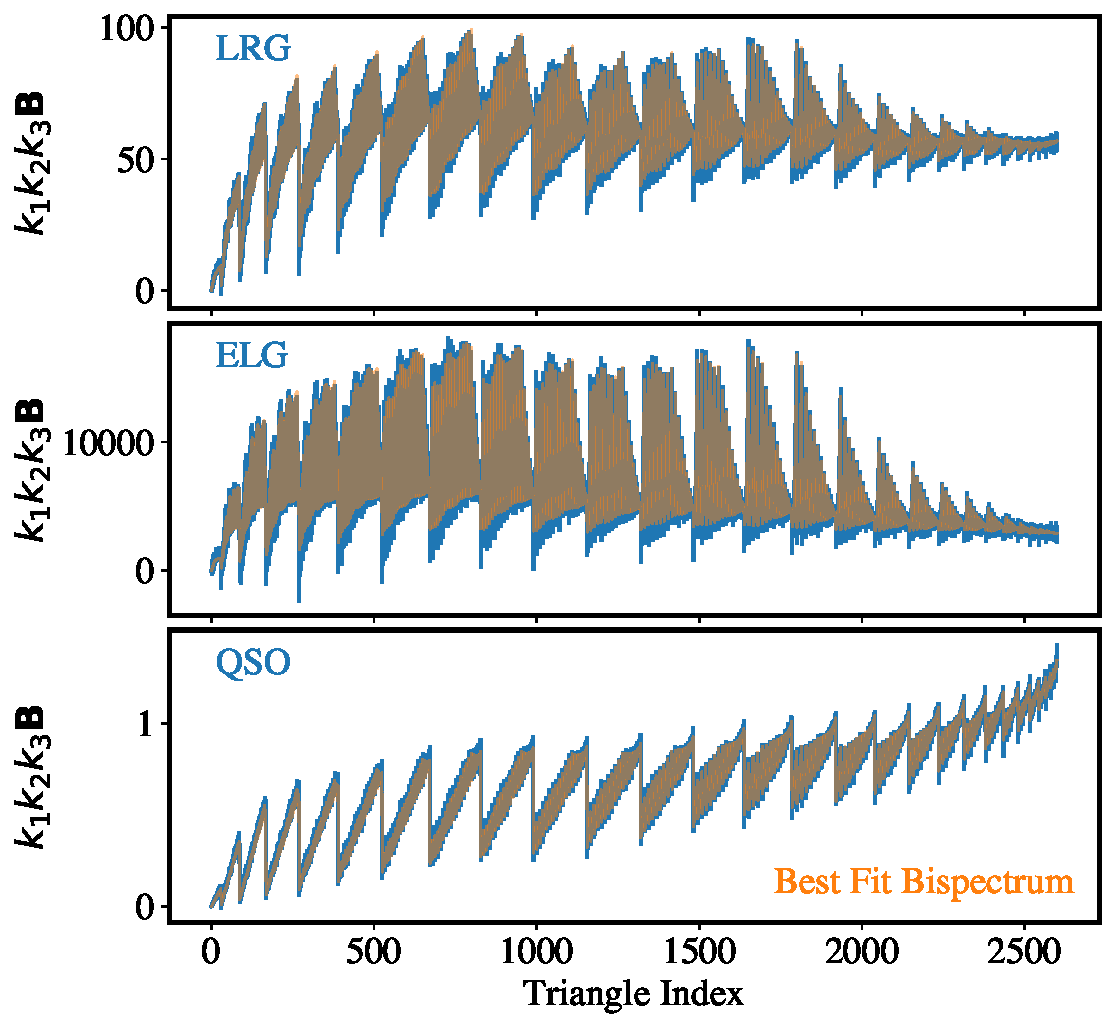
\includegraphics[width=0.45\textwidth]{figures/spectra.pdf}
\caption{Mean bispectrum of the Abacus LRG, ELG, and QSO simulations, repsectively, from top to bottom.}\label{fig:spectra}
\end{figure}

\begin{figure}
    \centering
    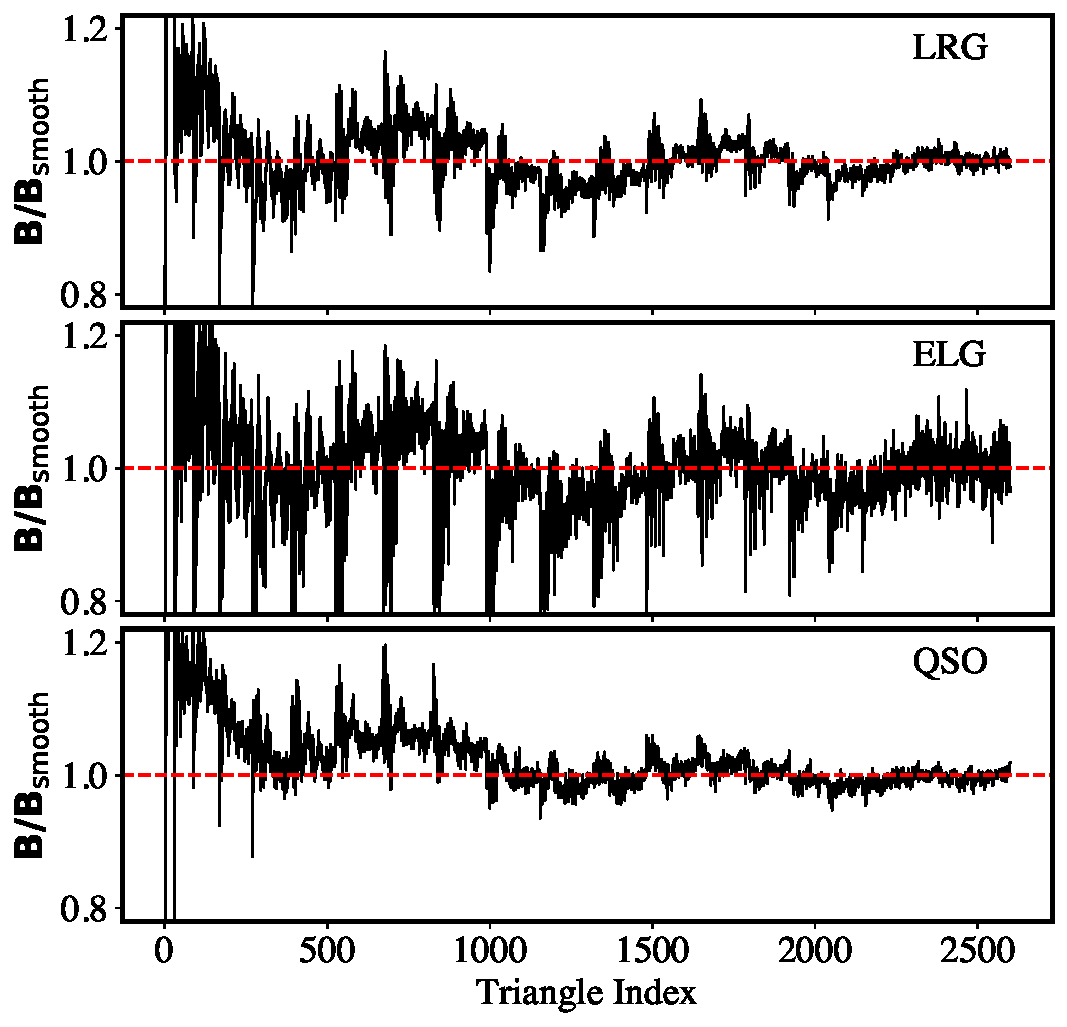
\includegraphics[width=0.45\textwidth]{figures/spectra_ratio.pdf}
    \caption{Same as Figure \ref{fig:spectra} for the ratio of bispectrum to smooth bispectrum.}
    \label{fig:spectra_ratio}
\end{figure}


\begin{figure}
    \centering
    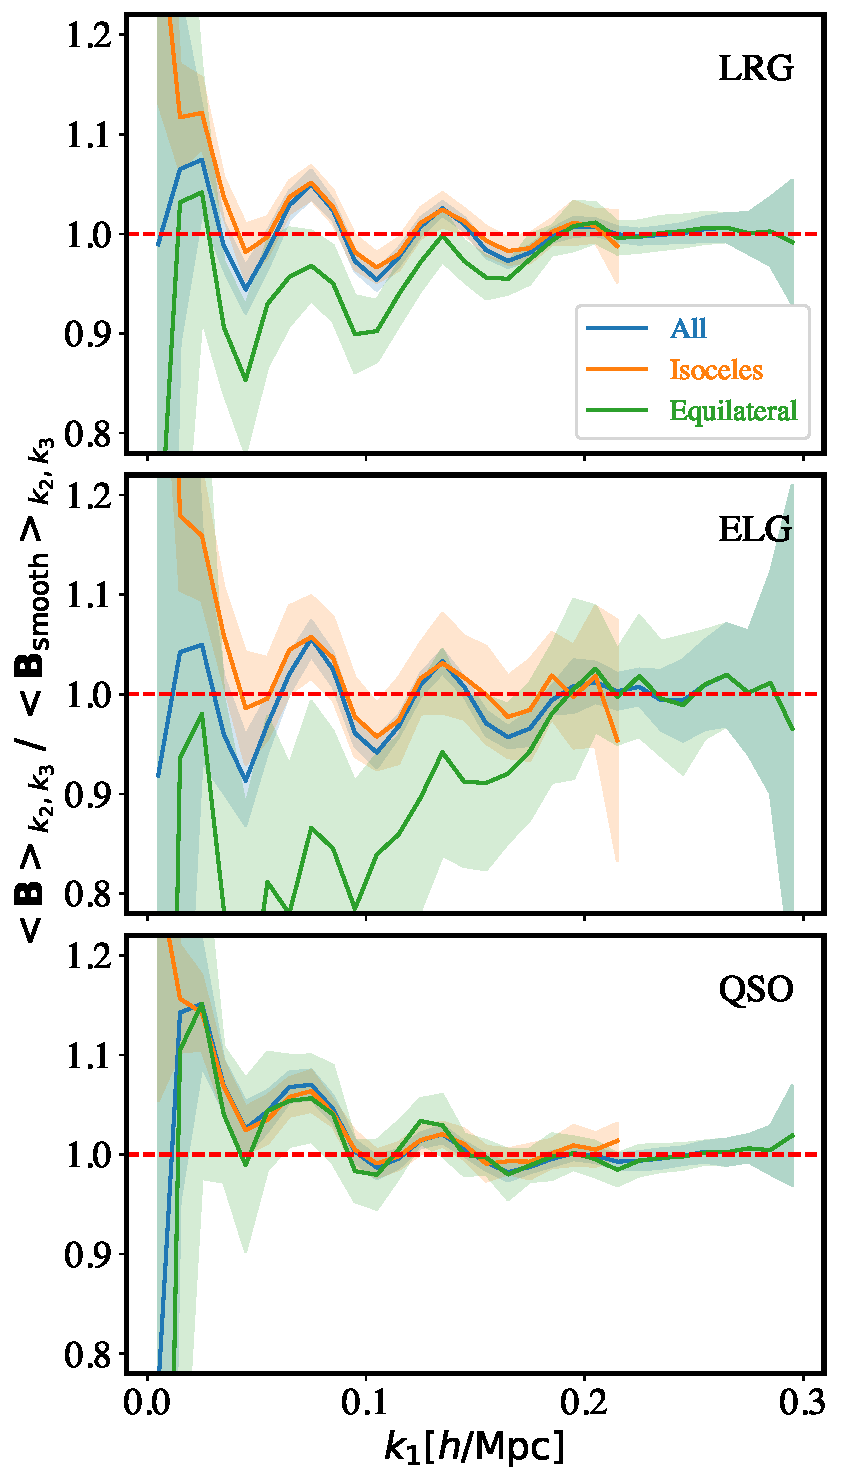
\includegraphics[width=0.45\textwidth]{figures/spectra_ratio_reduced.pdf}
    \caption{Same as Figure \ref{fig:spectra_ratio} for the reduced bispectrum.}
    \label{fig:spectra_ratio_reduced}
\end{figure}


\begin{figure}
    \centering
    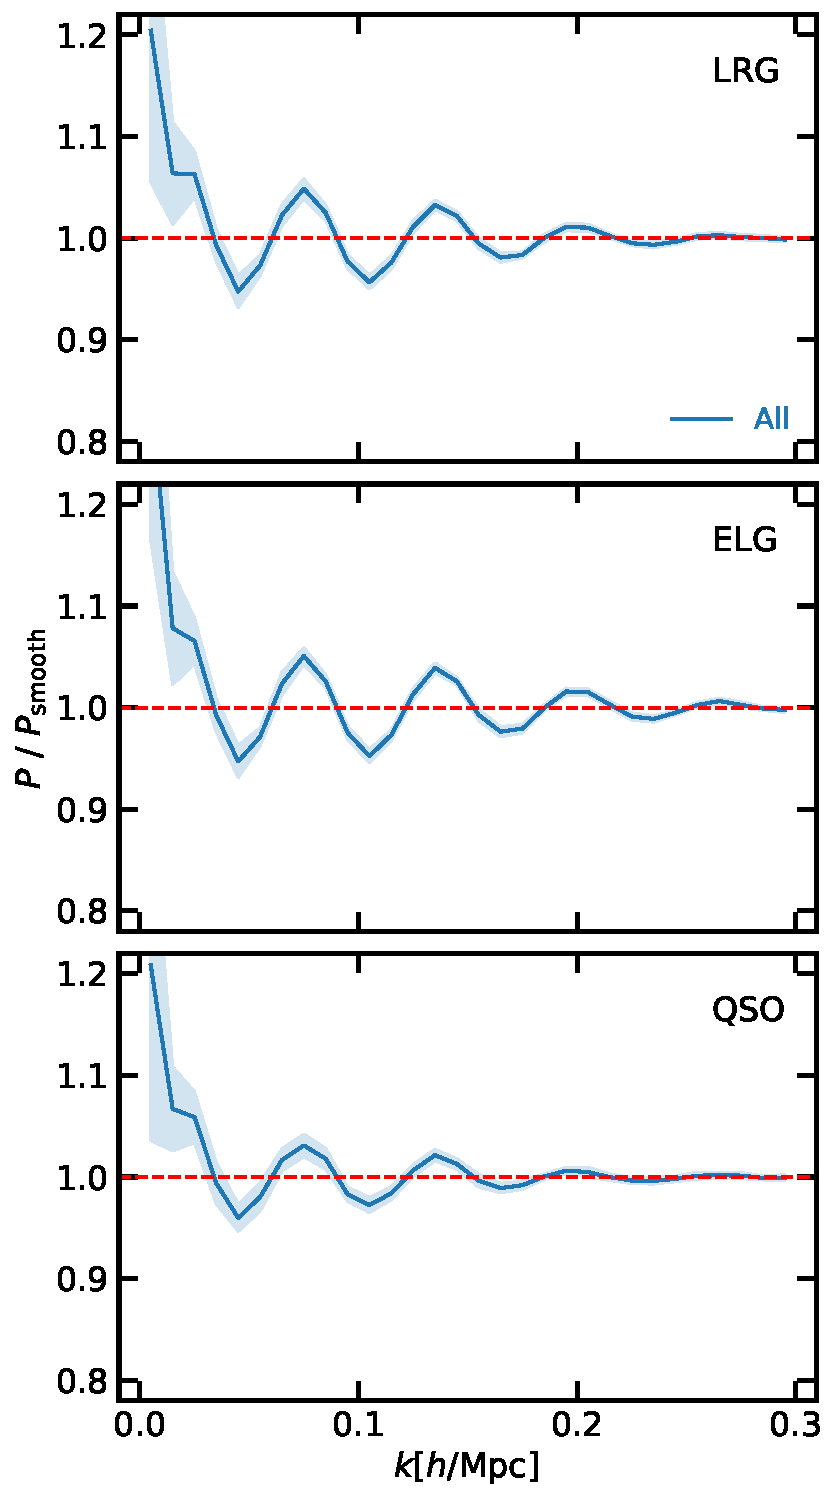
\includegraphics[width=0.45\textwidth]{figures/powerspectra_ratio.pdf}
    \caption{The ratio of the mean power spectrum to the mean smooth power spectrum.}
    \label{fig:powerspectra_ratio}
\end{figure}


\begin{figure*}
    \centering
    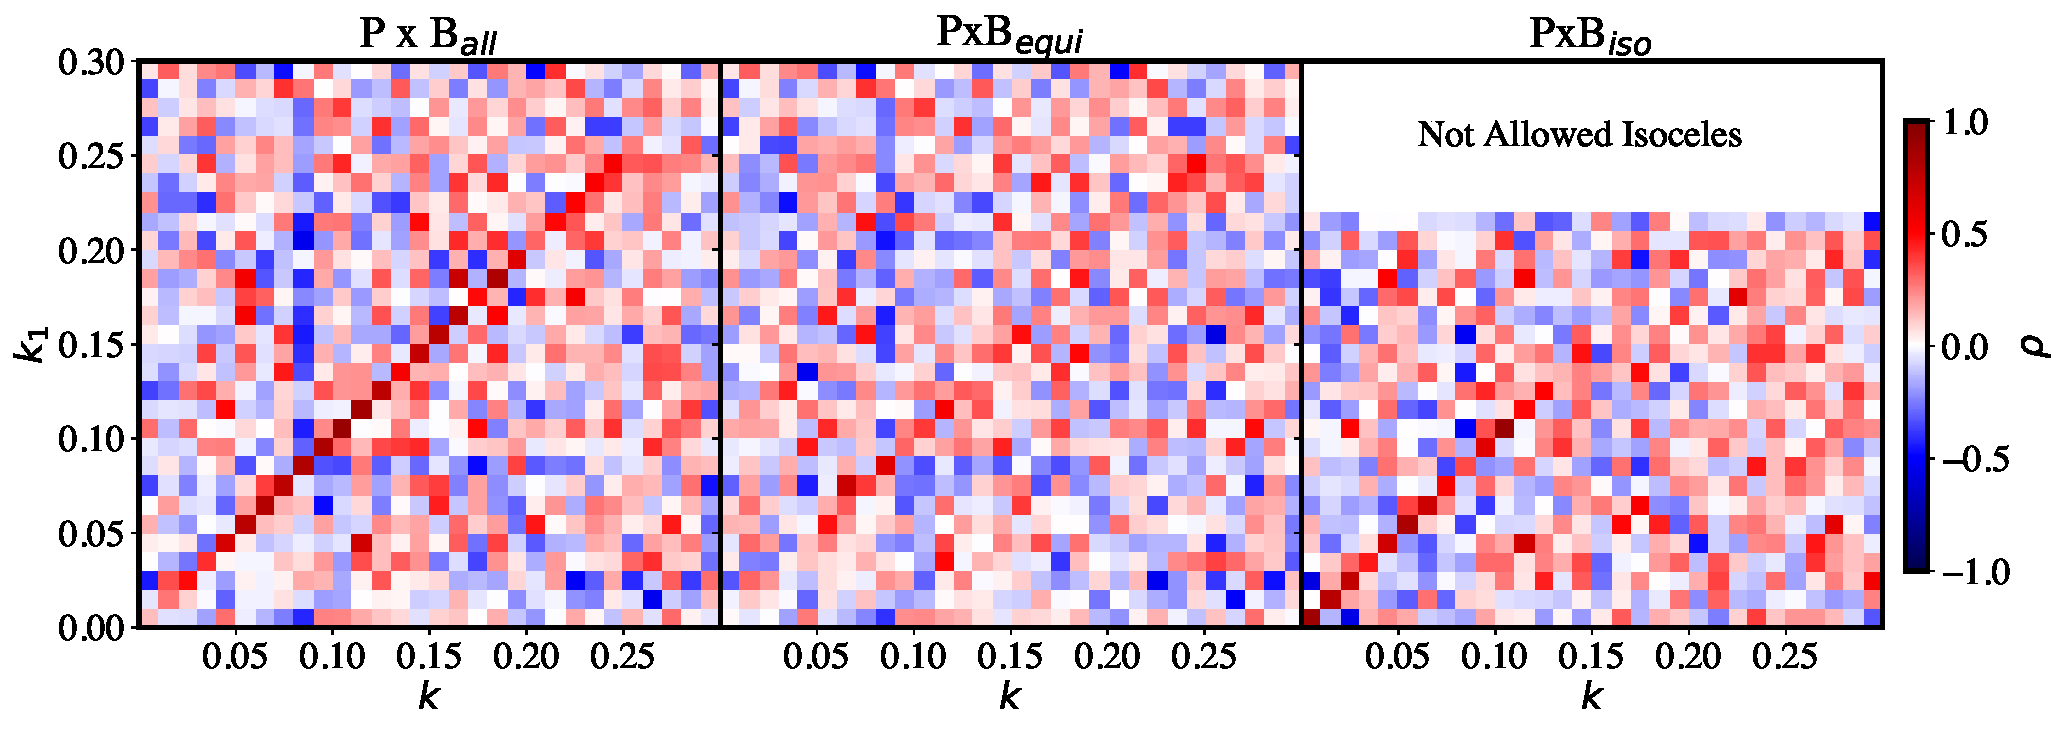
\includegraphics[width=\textwidth]{figures/corrmax_lrg.pdf}
    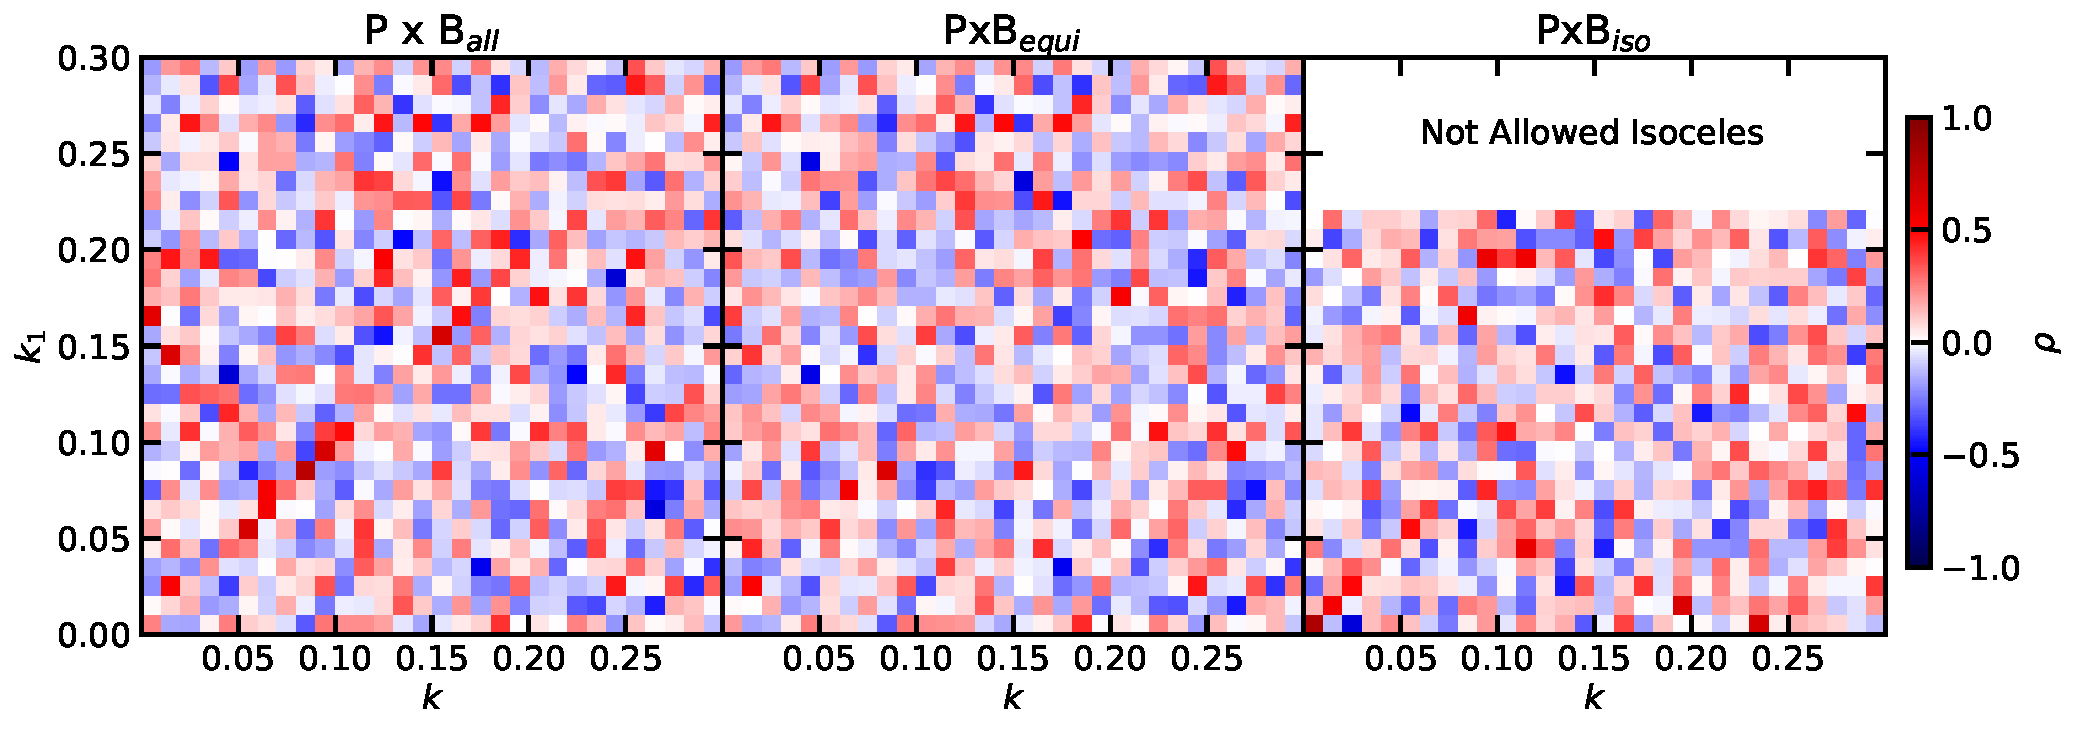
\includegraphics[width=\textwidth]{figures/corrmax_elg.pdf}
    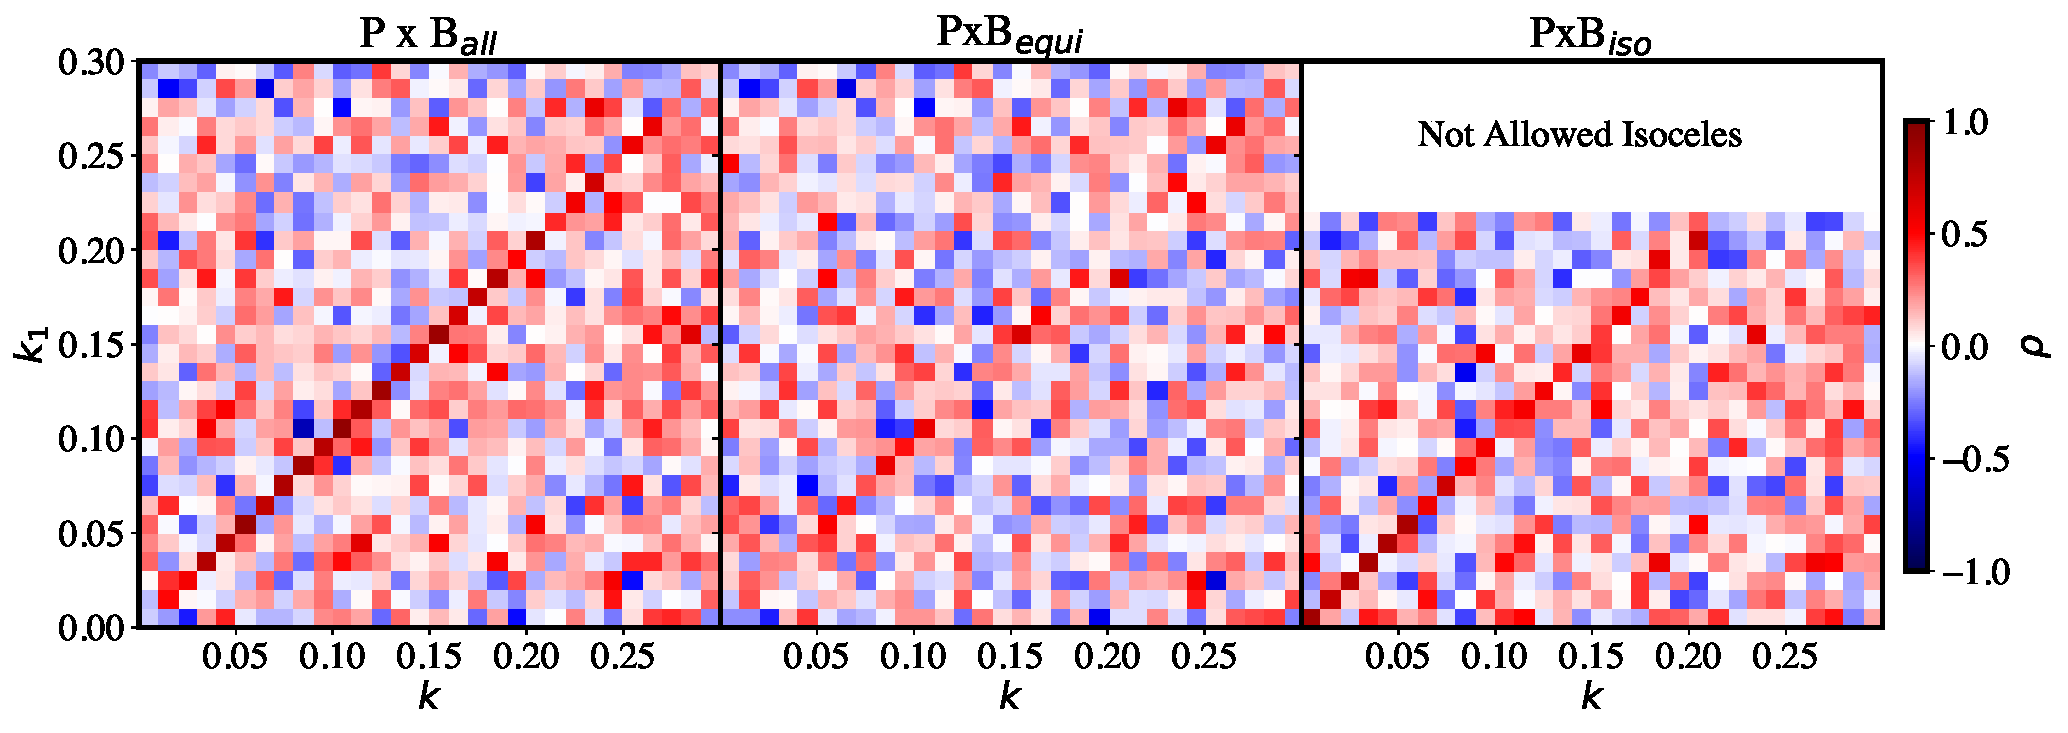
\includegraphics[width=\textwidth]{figures/corrmax_qso.pdf}
    \caption{The bin-by-bin cross-correlation of the reduced bispectrum and power spectrum measurements for ABACUS LRG, ELG, and QSO samples. The left to right panel show different bispectrum configurations, respectively, all, equilateral, and isosceles.}
    \label{fig:correlation}
\end{figure*}


\begin{figure*}
    \centering
    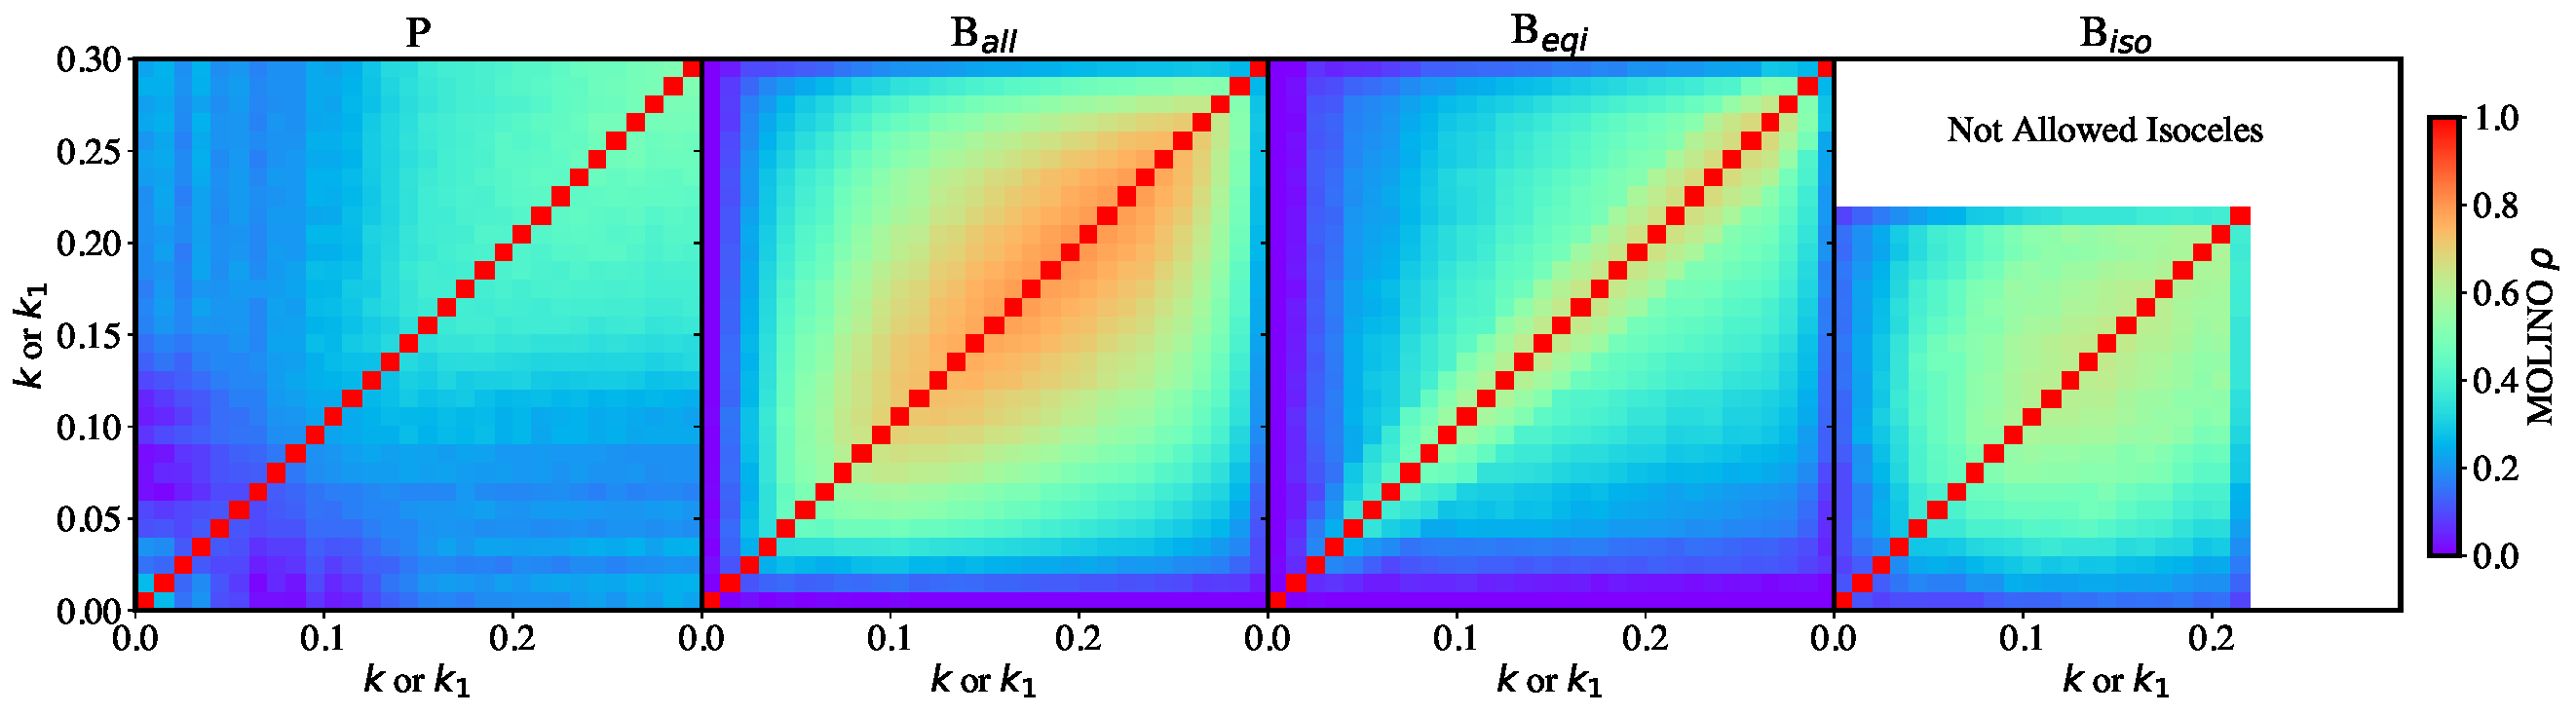
\includegraphics[width=\textwidth]{figures/corrmax_molino.pdf}
    \caption{Bin-by-bin auto-correlation of Molino power spectrum and reduced bispectrum.}
    \label{fig:correlation_molino}
\end{figure*}




\begin{figure*}
    \centering
    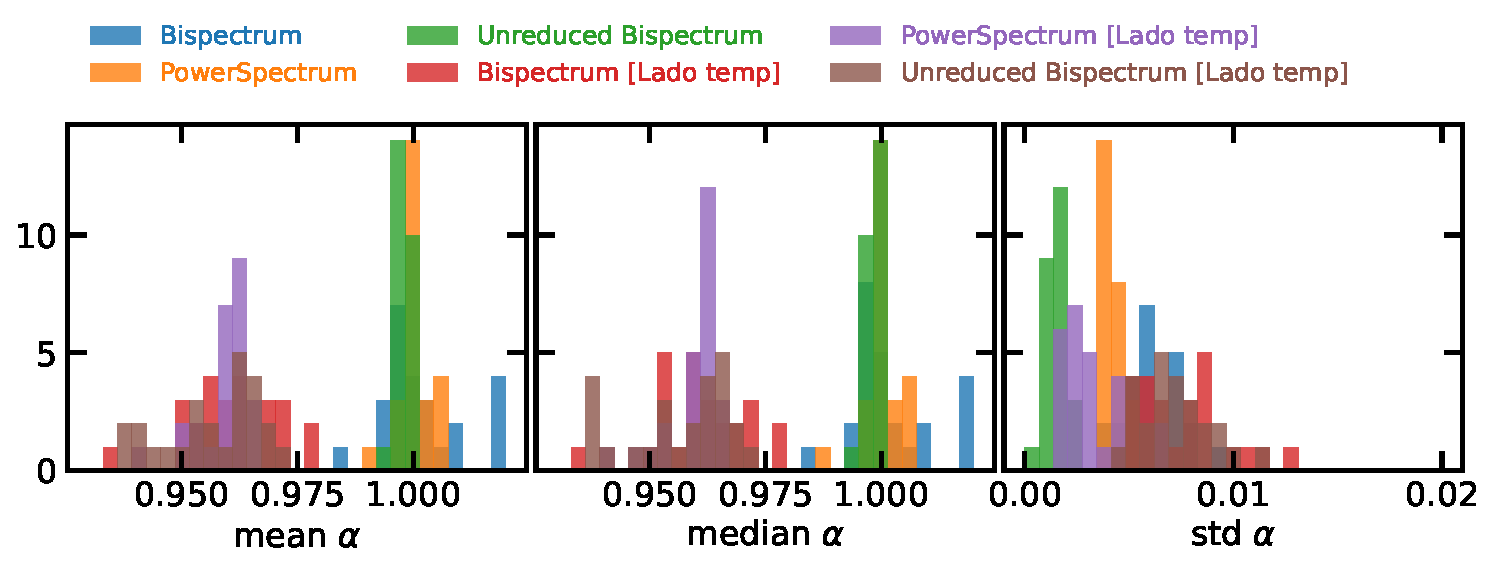
\includegraphics[width=\textwidth]{figures/constraints_LRGz0.pdf}
    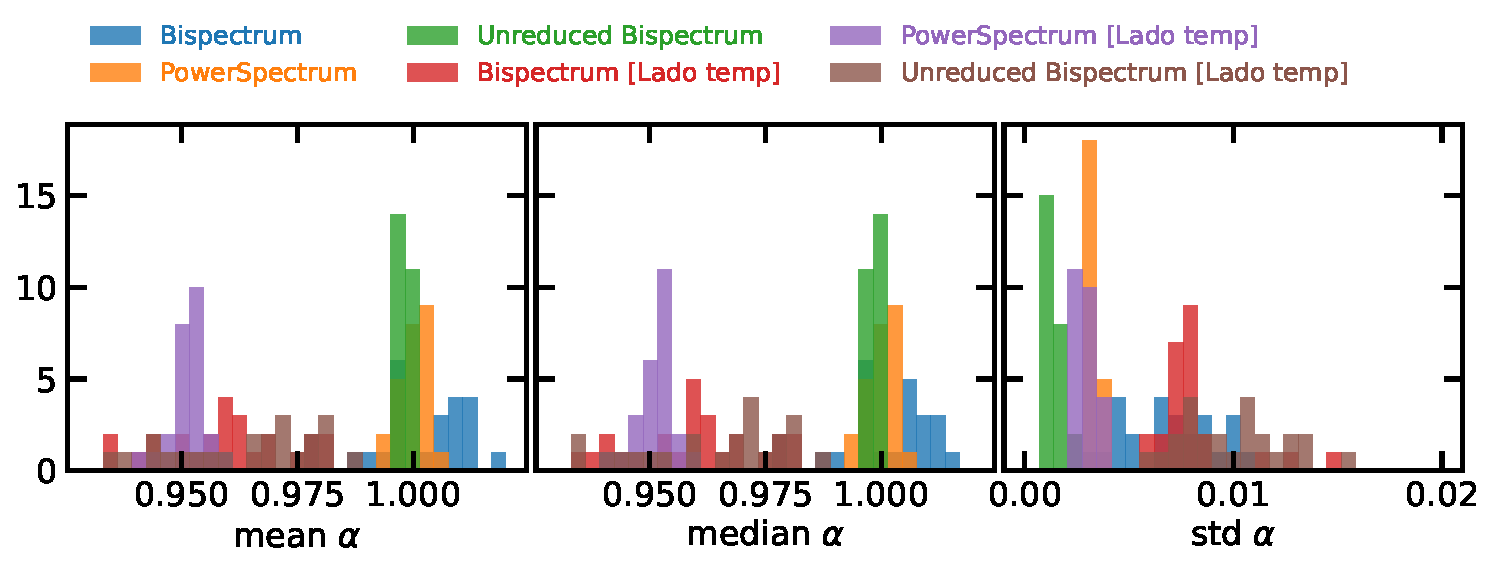
\includegraphics[width=\textwidth]{figures/constraints_ELGz1.pdf}
    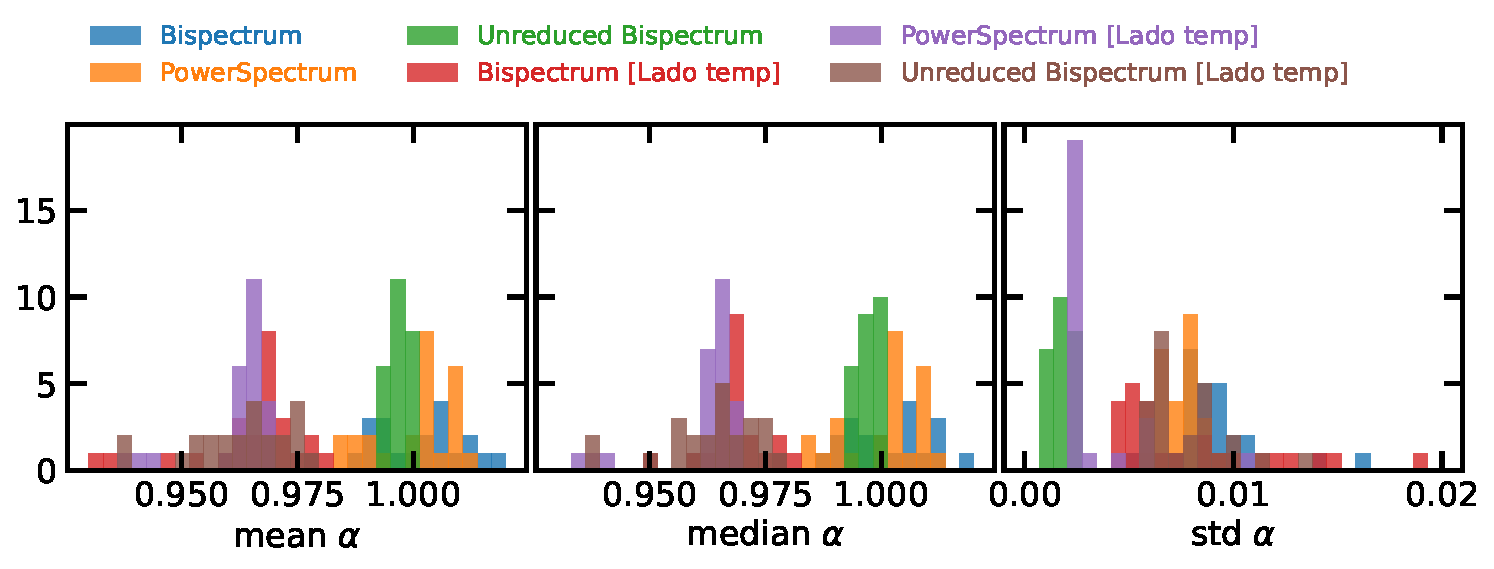
\includegraphics[width=\textwidth]{figures/constraints_QSOz2.pdf}    
    \caption{Mean, median, and standard deviation of BAO scale from 25 LRG (top), ELG (middle), and QSO (bottom) simulations.}
    \label{fig:constraints}
\end{figure*}


\begin{figure}
    \centering
    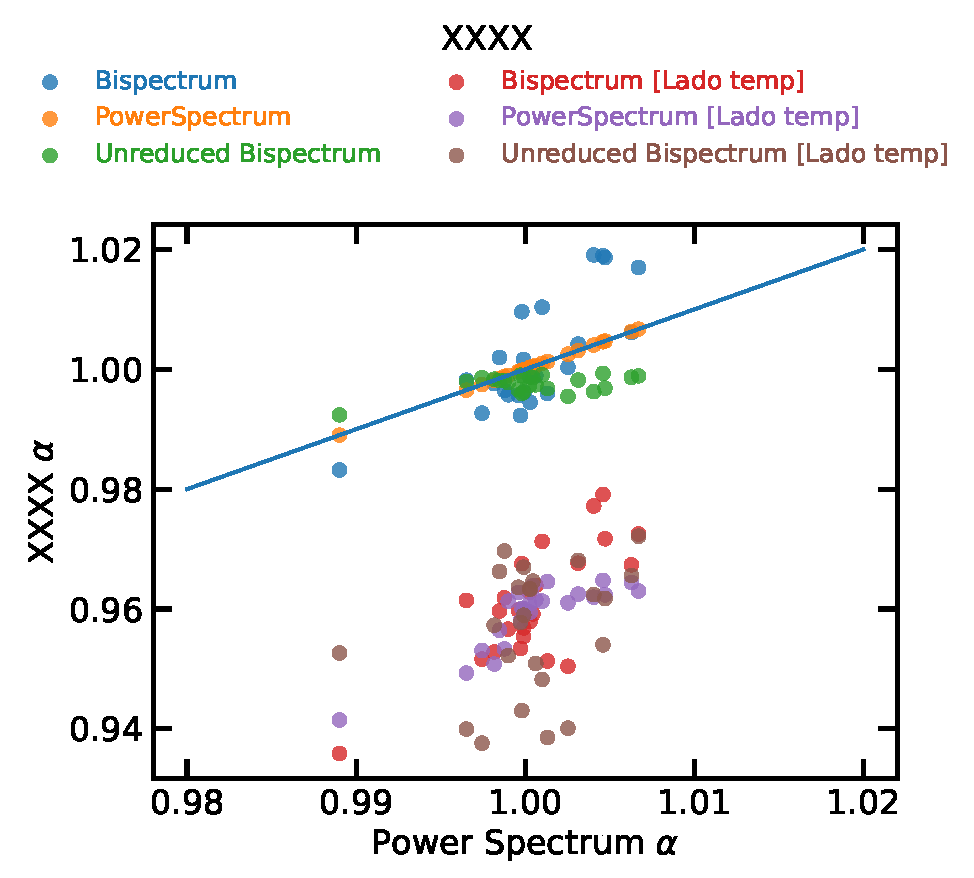
\includegraphics[width=0.45 \textwidth]{figures/constraints_scatter_LRGz0.pdf}
    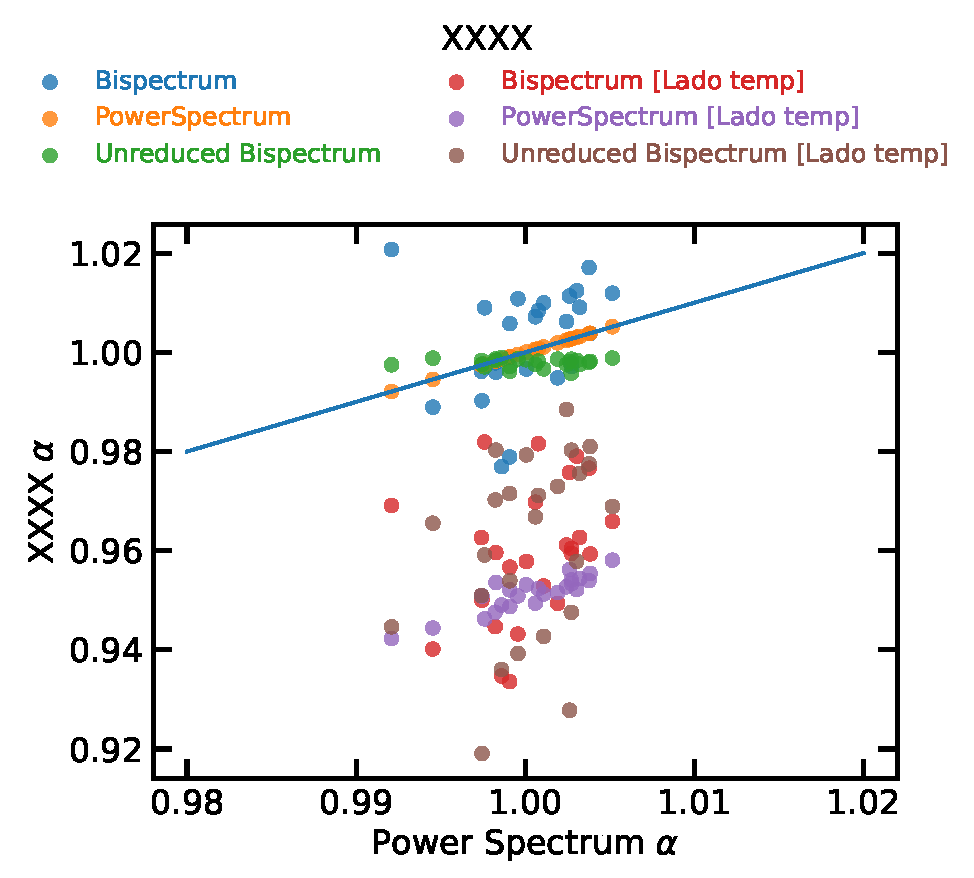
\includegraphics[width=0.45 \textwidth]{figures/constraints_scatter_ELGz1.pdf}
    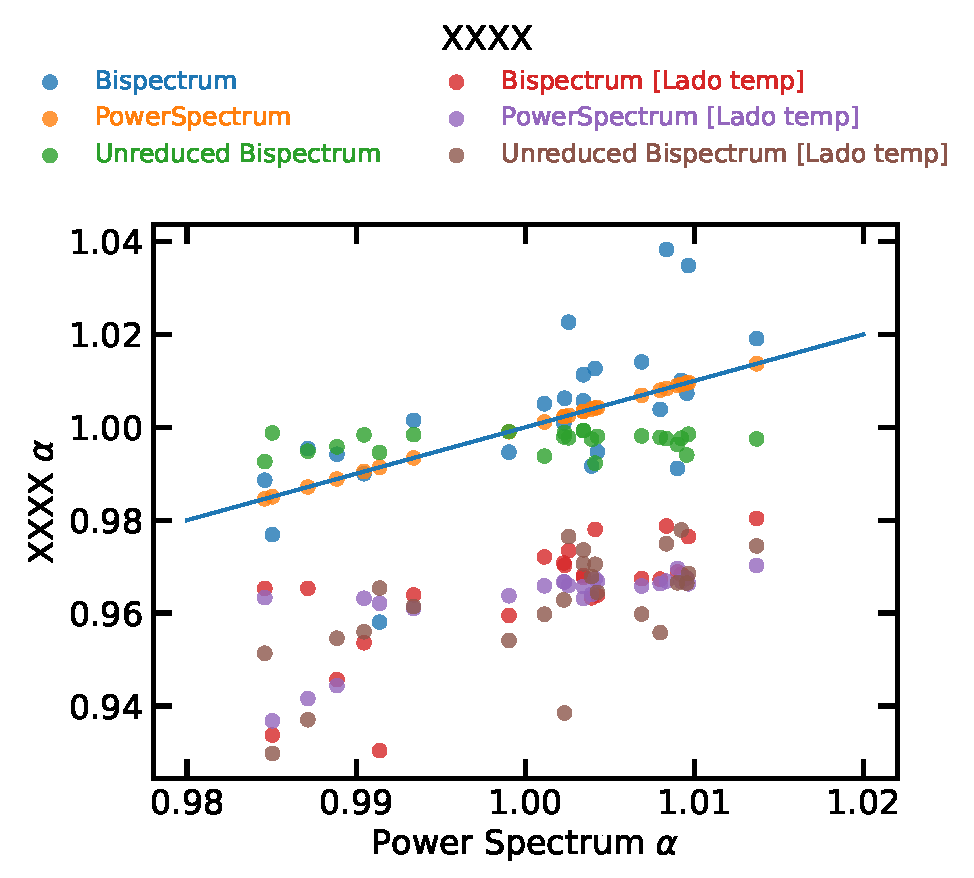
\includegraphics[width=0.45 \textwidth]{figures/constraints_scatter_QSOz2.pdf}
    \caption{BAO scale from various measurements vs that of power spectrum for 25 LRG (top), ELG (middle), and QSO (bottom) simulations.}
    \label{fig:scatter_cons}
\end{figure}